% UCL Thesis LaTeX Template
%  (c) Ian Kirker, 2014
% 
% This is a template/skeleton for PhD/MPhil/MRes theses.
%
% It uses a rather split-up file structure because this tends to
%  work well for large, complex documents.
% We suggest using one file per chapter, but you may wish to use more
%  or fewer separate files than that.
% We've also separated out various bits of configuration into their
%  own files, to keep everything neat.
% Note that the \input command just streams in whatever file you give
%  it, while the \include command adds a page break, and does some
%  extra organisation to make compilation faster. Note that you can't
%  use \include inside an \include-d file.
% We suggest using \input for settings and configuration files that
%  you always want to use, and \include for each section of content.
% If you do that, it also means you can use the \includeonly statement
%  to only compile up the section you're currently interested in.
% You might also want to put figures into their own files to be \input.

% For more information on \input and \include, see:
%  http://tex.stackexchange.com/questions/246/when-should-i-use-input-vs-include


% Formatting rules for theses are here: 
%  http://www.ucl.ac.uk/current-students/research_degrees/thesis_formatting
% Binding and submitting guidelines are here:
%  http://www.ucl.ac.uk/current-students/research_degrees/thesis_binding_submission

% This package goes first and foremost, because it checks all 
%  your syntax for mistakes and some old-fashioned LaTeX commands.
% Note that normally you Should load your documentclass before 
%  packages, because some packages change behaviour based on
%  your document settings.
% Also, for those confused by the RequirePackage here vs usepackage
%  elsewhere, usepackage cannot be used before the documentclass
%  command, while RequirePackage can. That's the only functional
%  difference as far as I'm aware.
\RequirePackage[l2tabu, orthodox]{nag}


% ------ Main document class specification ------
% The draft option here prevents images being inserted,
%  and adds chunky black bars to boxes that are exceeding 
%  the page width (to show that they are).
% The oneside option can optionally be replaced by twoside if
%  you intend to print double-sided. Note that this is
%  *specifically permitted* by the UCL thesis formatting
%  guidelines.
%
% Valid options in terms of type are:
%  phd
%  mres
%  mphil
%\documentclass[12pt,phd,draft,a4paper,oneside]{ucl_thesis}
\documentclass[11pt,phd,a4paper,oneside]{ucl_thesis}

% Package configuration:
%  LaTeX uses "packages" to add extra commands and features.
%  There are quite a few useful ones, so we've put them in a 
%   separate file.
% -------- Packages --------

% This package just gives you a quick way to dump in some sample text.
% You can remove it -- it's just here for the examples.
\usepackage{blindtext}

% This package means empty pages (pages with no text) won't get stuff
%  like chapter names at the top of the page. It's mostly cosmetic.
\usepackage{emptypage}

% The graphicx package adds the \includegraphics command,
%  which is your basic command for adding a picture.
\usepackage{graphicx}

% The float package improves LaTeX's handling of floats,
%  and also adds the option to *force* LaTeX to put the float
%  HERE, with the [H] option to the float environment.
\usepackage{float}

% The amsmath package enhances the various ways of including
%  maths, including adding the align environment for aligned
%  equations.
\usepackage{amsmath}

% Use these two packages together -- they define symbols
%  for e.g. units that you can use in both text and math mode.
\usepackage{gensymb}
\usepackage{textcomp}
% You may also want the units package for making little
%  fractions for unit specifications.
%\usepackage{units}


% The setspace package lets you use 1.5-sized or double line spacing.
\usepackage{setspace}
\setstretch{1.5}

% That just does body text -- if you want to expand *everything*,
%  including footnotes and tables, use this instead:
%\renewcommand{\baselinestretch}{1.5}


% PGFPlots is either a really clunky or really good way to add graphs
%  into your document, depending on your point of view.
% There's waaaaay too much information on using this to cover here,
%  so, you might want to start here:
%   http://pgfplots.sourceforge.net/
%  or here:
%   http://pgfplots.sourceforge.net/pgfplots.pdf
%\usepackage{pgfplots}
%\pgfplotsset{compat=1.3} % <- this fixed axis labels in the version I was using

% PGFPlotsTable can help you make tables a little more easily than
%  usual in LaTeX.
% If you're going to have to paste data in a lot, I'd suggest using it.
%  You might want to start with the manual, here:
%  http://pgfplots.sourceforge.net/pgfplotstable.pdf
%\usepackage{pgfplotstable}

% These settings are also recommended for using with pgfplotstable.
%\pgfplotstableset{
%	% these columns/<colname>/.style={<options>} things define a style
%	% which applies to <colname> only.
%	empty cells with={--}, % replace empty cells with '--'
%	every head row/.style={before row=\toprule,after row=\midrule},
%	every last row/.style={after row=\bottomrule}
%}


% The mhchem package provides chemistry formula typesetting commands
%  e.g. \ce{H2O}
%\usepackage[version=3]{mhchem}

% And the chemfig package gives a weird command for adding Lewis 
%  diagrams, for e.g. organic molecules
%\usepackage{chemfig}

% The linenumbers command from the lineno package adds line numbers
%  alongside your text that can be useful for discussing edits 
%  in drafts.
% Remove or comment out the command for proper versions.
%\usepackage[modulo]{lineno}
% \linenumbers 


% Alternatively, you can use the ifdraft package to let you add
%  commands that will only be used in draft versions
%\usepackage{ifdraft}

% For example, the following adds a watermark if the draft mode is on.
%\ifdraft{
%  \usepackage{draftwatermark}
%  \SetWatermarkText{\shortstack{\textsc{Draft Mode}\\ \strut \\ \strut \\ \strut}}
%  \SetWatermarkScale{0.5}
%  \SetWatermarkAngle{90}
%}


% The multirow package adds the option to make cells span 
%  rows in tables.
\usepackage{multirow}


% Subfig allows you to create figures within figures, to, for example,
%  make a single figure with 4 individually labeled and referenceable
%  sub-figures.
% It's quite fiddly to use, so check the documentation.
%\usepackage{subfig}

% The natbib package allows book-type citations commonly used in
%  longer works, and less commonly in science articles (IME).
% e.g. (Saucer et al., 1993) rather than [1]
% More details are here: http://merkel.zoneo.net/Latex/natbib.php
%\usepackage{natbib}

% The bibentry package (along with the \nobibliography* command)
%  allows putting full reference lines inline.
%  See: 
%   http://tex.stackexchange.com/questions/2905/how-can-i-list-references-from-bibtex-file-in-line-with-commentary
\usepackage{bibentry} 

% The isorot package allows you to put things sideways 
%  (or indeed, at any angle) on a page.
% This can be useful for wide graphs or other figures.
%\usepackage{isorot}

% The caption package adds more options for caption formatting.
% This set-up makes hanging labels, makes the caption text smaller
%  than the body text, and makes the label bold.
% Highly recommended.
\usepackage[format=hang,font=small,labelfont=bf]{caption}

% If you're getting into defining your own commands, you might want
%  to check out the etoolbox package -- it defines a few commands
%  that can make it easier to make commands robust.
\usepackage{etoolbox}


% Sets up links within your document, for e.g. contents page entries
%  and references, and also PDF metadata.
% You should edit this!
%%
%% This file uses the hyperref package to make your thesis have metadata embedded in the PDF, 
%%  and also adds links to be able to click on references and contents page entries to go to 
%%  the pages.
%%

% Some hacks are necessary to make bibentry and hyperref play nicely.
% See: http://tex.stackexchange.com/questions/65348/clash-between-bibentry-and-hyperref-with-bibstyle-elsart-harv
\usepackage{bibentry}
\makeatletter\let\saved@bibitem\@bibitem\makeatother
\usepackage[pdftex,hidelinks]{hyperref}
\makeatletter\let\@bibitem\saved@bibitem\makeatother
\makeatletter
\AtBeginDocument{
    \hypersetup{
        pdfsubject={Thesis Subject},
        pdfkeywords={Thesis Keywords},
        pdfauthor={Author},
        pdftitle={Title},
    }
}
\makeatother
    


% And then some settings in separate files.
% These settings are from:
%  http://mintaka.sdsu.edu/GF/bibliog/latex/floats.html

% They give LaTeX more options on where to put your figures, and may
%  mean that fewer of your figures end up at the tops of pages far
%  away from the thing they're related to.

% Alters some LaTeX defaults for better treatment of figures:
% See p.105 of "TeX Unbound" for suggested values.
% See pp. 199-200 of Lamport's "LaTeX" book for details.

%   General parameters, for ALL pages:
\renewcommand{\topfraction}{0.9}	% max fraction of floats at top
\renewcommand{\bottomfraction}{0.8}	% max fraction of floats at bottom

%   Parameters for TEXT pages (not float pages):
\setcounter{topnumber}{2}
\setcounter{bottomnumber}{2}
\setcounter{totalnumber}{4}     % 2 may work better
\setcounter{dbltopnumber}{2}    % for 2-column pages
\renewcommand{\dbltopfraction}{0.9}	% fit big float above 2-col. text
\renewcommand{\textfraction}{0.07}	% allow minimal text w. figs

%   Parameters for FLOAT pages (not text pages):
\renewcommand{\floatpagefraction}{0.7}	% require fuller float pages
% N.B.: floatpagefraction MUST be less than topfraction !!
\renewcommand{\dblfloatpagefraction}{0.7}	% require fuller float pages

% remember to use [htp] or [htpb] for placement,
% e.g. 
%  \begin{figure}[htp]
%   ...
%  \end{figure} % For things like figures and tables
\bibliographystyle{unsrt}   % For bibliographies

% These control how many number sections your subsections will take
%    e.g. Section 2.3.1.5.6.3
%  and how many of those will get put into the contents pages.
\setcounter{secnumdepth}{3}
\setcounter{tocdepth}{3}


\begin{document}

\nobibliography*
% ^-- This is a dumb trick that works with the bibentry package to let
%  you put bibliography entries whereever you like.
% I used this to put references to papers a chapter's work was 
%  published in at the end of that chapter.
% For more information, see: http://stefaanlippens.net/bibentry

% If you haven't finished making your full BibTex file yet, you
%  might find this useful -- it'll just replace all your
%  citations with little superscript notes.
% Uncomment to use.
\renewcommand{\cite}[1]{\emph{\textsuperscript{[#1]}}}
%\parindent=0pt%don't indent paragraphs
% At last, content! Remember filenames are case-sensitive and 
%  *must not* include spaces.
% I may change the way this is done in a future version, 
%  but given that some people needed it, if you need a different degree title 
%  (e.g. Master of Science, Master in Science, Master of Arts, etc)
%  uncomment the following 3 lines and set as appropriate (this *has* to be before \maketitle)
\makeatletter
\renewcommand {\@degree@string}{Music Computing}
\makeatother

\title{Parameter automation for granular synthesis}
\author{Karol Bakunowski}
\department{Department of Computing}

\maketitle
%\makedeclaration

\begin{abstract} % 300 word limit
My research is about stuff.

It begins with a study of some stuff, and then some other stuff and things.

There is a 300-word limit on your abstract.

    A good abstract explains in one line why the paper is important. It then goes on to give a summary of your major results, preferably couched in numbers with error limits. The final sentences explain the major implications of your work. A good abstract is concise, readable, and quantitative. 
    Length should be ~ 1-2 paragraphs, approx. 400 words.
    Absrtracts generally do not have citations.
    Information in title should not be repeated. 
    Be explicit. 
    Use numbers where appropriate.
    Answers to these questions should be found in the abstract: 
        What did you do? 
        Why did you do it? What question were you trying to answer? 
        How did you do it? State methods.
        What did you learn? State major results. 
        Why does it matter? Point out at least one significant implication.

\end{abstract}

\iffalse
\begin{comment}
\begin{impactstatement}

	UCL theses now have to include an impact statement. \textit{(I think for REF reasons?)} The following text is the description from the guide linked from the formatting and submission website of what that involves. (Link to the guide: {\scriptsize \url{http://www.grad.ucl.ac.uk/essinfo/docs/Impact-Statement-Guidance-Notes-for-Research-Students-and-Supervisors.pdf}})

\begin{quote}
The statement should describe, in no more than 500 words, how the expertise, knowledge, analysis,
discovery or insight presented in your thesis could be put to a beneficial use. Consider benefits both
inside and outside academia and the ways in which these benefits could be brought about.

The benefits inside academia could be to the discipline and future scholarship, research methods or
methodology, the curriculum; they might be within your research area and potentially within other
research areas.

The benefits outside academia could occur to commercial activity, social enterprise, professional
practice, clinical use, public health, public policy design, public service delivery, laws, public
discourse, culture, the quality of the environment or quality of life.

The impact could occur locally, regionally, nationally or internationally, to individuals, communities or
organisations and could be immediate or occur incrementally, in the context of a broader field of
research, over many years, decades or longer.

Impact could be brought about through disseminating outputs (either in scholarly journals or
elsewhere such as specialist or mainstream media), education, public engagement, translational
research, commercial and social enterprise activity, engaging with public policy makers and public
service delivery practitioners, influencing ministers, collaborating with academics and non-academics
etc.

Further information including a searchable list of hundreds of examples of UCL impact outside of
academia please see \url{https://www.ucl.ac.uk/impact/}. For thousands more examples, please see
\url{http://results.ref.ac.uk/Results/SelectUoa}.
\end{quote}
\end{impactstatement}
\fi

\begin{acknowledgements}
Acknowledge all the things!
\end{acknowledgements}

\setcounter{tocdepth}{2} 
% Setting this higher means you get contents entries for
%  more minor section headers.

\tableofcontents
\listoffigures
\listoftables
\chapter{Introduction}
\label{chapterlabel1}

\section{Aims and Objectives}
%i should consider writing a 'hook' sentence/paragraph here to draw readers
%attention and make them interested in the rest of the paper
The initial aim of the project was to implement a machine learning solution to
the task of granular synthesizer programming based on sound matching.
Consequently building a tool that would assist musicians in creating interesting
sounds, provided an audio input to the system.

Over the course of the past couple months the project extended into more
research-oriented directions, with a focus of finding the best possible audio
descriptors for specific characteristics of sounds. In order to determine the
most significant in judging similarity on the cognitive level.

The methods here concerned with describing audio differ from other approaches in
literature (e.g Matthew) primarily in that sound is treated in a modular manner,
where a description is made based on one characteristic for X number instances,
and separate processes are run for each. Instead of trying to describe audio as
a whole, the aim is to describe it as a combination of things (density, pitch,
rhythm, amplitude)

Concretely my objectives are:

1. To build a tool that is helpful to artists in creating new sounds 

2. To challenge the interaction between an artist and a preset as a starting
point to synthesis 

3. To achieve a response that is not only stimulating to the user but also differs
from simply randomizing the parameter values 

In measuring the project's success, the subjective sonic coherence and
similarity of algorithm's outputs may be considered the best indicator (the
human discriminator?), along with more quantitative analysis, such as comparing
the audio descriptors on input and output sounds for example.

In (future chapters) I provide some critique on established techniques of
assessment of these types of problems and ultimately conclude that some stuff in
the best way of doing it.

\subsection{Deliverables}
to these ends hehhe this is what i made:

Some stuff about things.\cite{example-citation} Some more things. 
Inline citation: \bibentry{example-citation}

\iffalse
This section should be about 500 words.

You can't write a good introduction until you know what the body of the paper says. Consider writing the introductory section(s) after you have completed the rest of the paper, rather than before.


Be sure to include a hook at the beginning of the introduction. This is a statement of something sufficiently interesting to motivate your reader to read the rest of the paper, it is an important/interesting scientific problem that your paper either solves or addresses. You should draw the reader in and make them want to read the rest of the paper.

The next paragraphs in the introduction should cite previous research in this area. It should cite those who had the idea or ideas first, and should also cite those who have done the most recent and relevant work. You should then go on to explain why more work was necessary (your work, of course.)
 
What else belongs in the introductory section(s) of your paper? 

1.    A statement of the goal of the paper: why the study was undertaken, or why the paper was written. Do not repeat the abstract. 

2.   Sufficient background information to allow the reader to understand the context and significance of the question you are trying to address. 

3. Proper acknowledgement of the previous work on which you are building.
Sufficient references such that a reader could, by going to the library, achieve
a sophisticated understanding of the context and significance of the question.

4.    The introduction should be focused on the thesis question(s).  All cited work should be directly relevant to the goals of the thesis.  This is not a place to summarize everything you have ever read on a subject.

5.    Explain the scope of your work, what will and will not be included. 

6.    A verbal "road map" or verbal "table of contents" guiding the reader to what lies ahead. 

7.    Is it obvious where introductory material ("old stuff") ends and your contribution ("new stuff") begins? 

Remember that this is not a review paper. We are looking for original work and interpretation/analysis by you. Break up the introduction section into logical segments by using subheads. 
\fi
\chapter{Literature Review}

\section{Problem background}

Mimicking sounds is very intuitive for humans. Humming along a song
we've heard previously, or generally repeating something so that it
sounds as close to the original as possible seems like a rather
trivial task for us. However, musicians who are able to translate what
they hear in their head, directly to an instrument, be it a physical
one like piano or guitar, or a software based instrument, are
considered viruosic.

Yet, many successful musicians might be programming synthesizers
following a not clearly defined `intuition', and often look for
inspiration for the sound they are trying to create.
% \cite{noauthor_oneohtrix_2016} \cite{herbert_manifesto_2011}
Especially today, a lot of sounds are created by the means of experimental
methods, often using presets as a starting point.

Therefore, to be able to replicate any sound in a synthesizer, based
only on an audio input would seem like a very intuitive way of
working, and interacting with synthesizers.

\subsection{Audio descriptors}

Unfortunately, based on how sound is represented digitally, mimicking
sounds is not as intuitive for computers as it is for humans. In order
to describe sounds we need some algorithms, that are capable of
generating meanigful data about given audio signal. A great amount of
these analysis tools exist, and generally they can be devided into two
categories. One dealing with timbre, and another dealing with rhythm,
or otherwise temoral qualities of the signal.

\subsubsection{Rhythm}

Onset detection, which tries to estimate how many `peaks' there are
in a signal is a very useful algorithm to estimate how much rhythmical
content there is present.

\subsubsection{Timbre}

In order to compute any sort of pitch detection, the audio signal has
to be translated from the time domain to the frequency domain. This
can be achieved by the inexplicably useful algorithm in music today: 
Fourier Transform. It can dissect a signal to it's most basic
sinusoidal components, therefore determining how much of which
frequencies are present in the signal, which in turn can directly
translate into pitch.

Building on that, possibly the most powerful algorithm for determining
the timbre of an audio signal is Mel-frequency cepstrum coefficients,
or MFCC. Many studies have been done to prove the usefullness of MFCCs
in describing the timbral, and as a matter of fact rythymical content
of audio signals. They are mainly used in speech symthesis and speech
recognition, however can be apply to any signal, and are a very
powerful descriptor.

\subsection{Granulation}

There is one, major limitation, when it comes to parameter predictions
for a granular, or any other corpus-based synthesizer. The sounds
created are heavily based on the sample fed into the synthesizer. Each
parameter changes meaning significantly, once the input sample is
changed. 

Two possible solutions come to mind, when trying to overcome this
problem. Using one input sample for synthesis, and trying
to predict samples for one perticular instance of the granulator is one.
Another, would be trying to fit some universal analysis algorithms,
that could decribe rhythym, pitch, density of sound etc. independently
of the original sample. This way any sample could be `molded' into
what would resemble the original prediction target. 

Concatenative synthesis is an alternative approach to this problem. It
could be beneficial, as it would try to find `grains' as closely
resembling parts of the target as possible, and recreate it using
little parts, almost like puzzles, that the algorithm thinks
fit. However, that approach also has limitations, as it could only
recreate the target sound out of the samples stored in it's database,
therefore making the output biased.

\subsection{Machine Learning (predictions?)}

A neural network could be used to build a parameter space for any
synthesizer from some input, which here would mean the audio analysis
algorithms results. A lot of research has been done on this
topic. From feedforward networks (cite) paired with analysis
algorithms, to Long Short Term Memory networks to take into account
the temporal information conveyed in different frames of the MFCC
analysis (citation). Convolutional networks are also very often used,
especially for classification of sounds.

Different algorithms were used previously to tackle the task of
automatic synthesizer programming, including Hill Climber (cite),
Genetic Algorithms (cite) etc.

Alternatively, in order to try and generalise the predictions for
different input samples for the synthesizer. The predictions could be
devided between different parameters. Then linking different
prediction algorithms with different parameters could possibly allow
for a creation of a more direct relationship between audio descriptors
and the synthesis results. 

%% ppr:
%Programming synthesizers is a fun, but challenging task. The range of sounds possible to
%achieve on such a device, and consequently the amount of adjustable parameters can be overwhelming.
%From choosing an audio file to sample, to an amplitude envelope for each grain, the ability to make
%decisions about programming a granulator has to come from either a place of certainty about what
%each parameter is responsible for, or a place of experimental thought, and a somewhat random
%parameter value assignments.

%Users fairly new in the realm of synthesizer programming may encounter issues creating sounds they
%desire. Even successful musicians might be doing things following a not clearly defined “intuition”.
%There are of course people who are experts in this field, but artists often look for inspiration
%when it comes to timbre of their sounds.
%%\cite{noauthor_oneohtrix_2016} \cite{herbert_manifesto_2011}
%It would seem that, the use of presets as a starting point is not unusual.

%My future thesis will aim to offer an alternative way to approach the creation of new sounds.

%%based on this write sections i think
%Research has been done previously as an investigation into automation of parameters in synthesizers
%based on sound matching. Taking a snippet of sound, the algorithm would try to
%find parameter settings to match a produced sound as closely as possible to the
%source%\cite{yee-king_automatic_2018}.

%This research mostly focuses on FM synthesis
%% \cite{horner_machine_1993}
%, although
%experiments on different synthesis techniques has been
%done
%% \cite{dahlstedt_creating_nodate}
%, including any VST
%plug-in
%% \cite{yee-king_synthbot:_nodate}.
%
%However, using this approach on corpus-based synthesis remains an untapped area
%of research, worth investigating
%%\cite{mcdonald_neural_2017}.
%
%Also, it seems that most of this research focuses on reproducing the original
%input
% \cite{tatar_automatic_2016}
%. Perhaps more interesting and novel sounds
%could arise as an effect of bad performance, but is does not seem to be the
%desired outcome in most cases.


%It seems like a description of this section is also in the introduction
%description. Which means that it could probably be fitted in there, instead of
%making a whole another section for it in the paper.

%% advice 

%The next paragraphs in the introduction should cite previous research in this
%area. It should cite those who had the idea or ideas first, and should also cite
%those who have done the most recent and relevant work. You should then go on to
%explain why more work was necessary (your work, of course.)

%Sufficient background information to allow the reader to understand the context
%and significance of the question you are trying to address.

%Proper acknowledgement of the previous work on which you are building.
%Sufficient references such that a reader could, by going to the library, achieve
%a sophisticated understanding of the context and significance of the question.

%The introduction should be focused on the thesis question(s). All cited work
%should be directly relevant to the goals of the thesis. This is not a place to
%summarize everything you have ever read on a subject.% lit review
\chapter{Methods}

The method of tackling this problem will be based on previous research done in this domain. There are three essential components for this project:
\begin{figure}[h]
\caption{Basic flowchart}
\centering
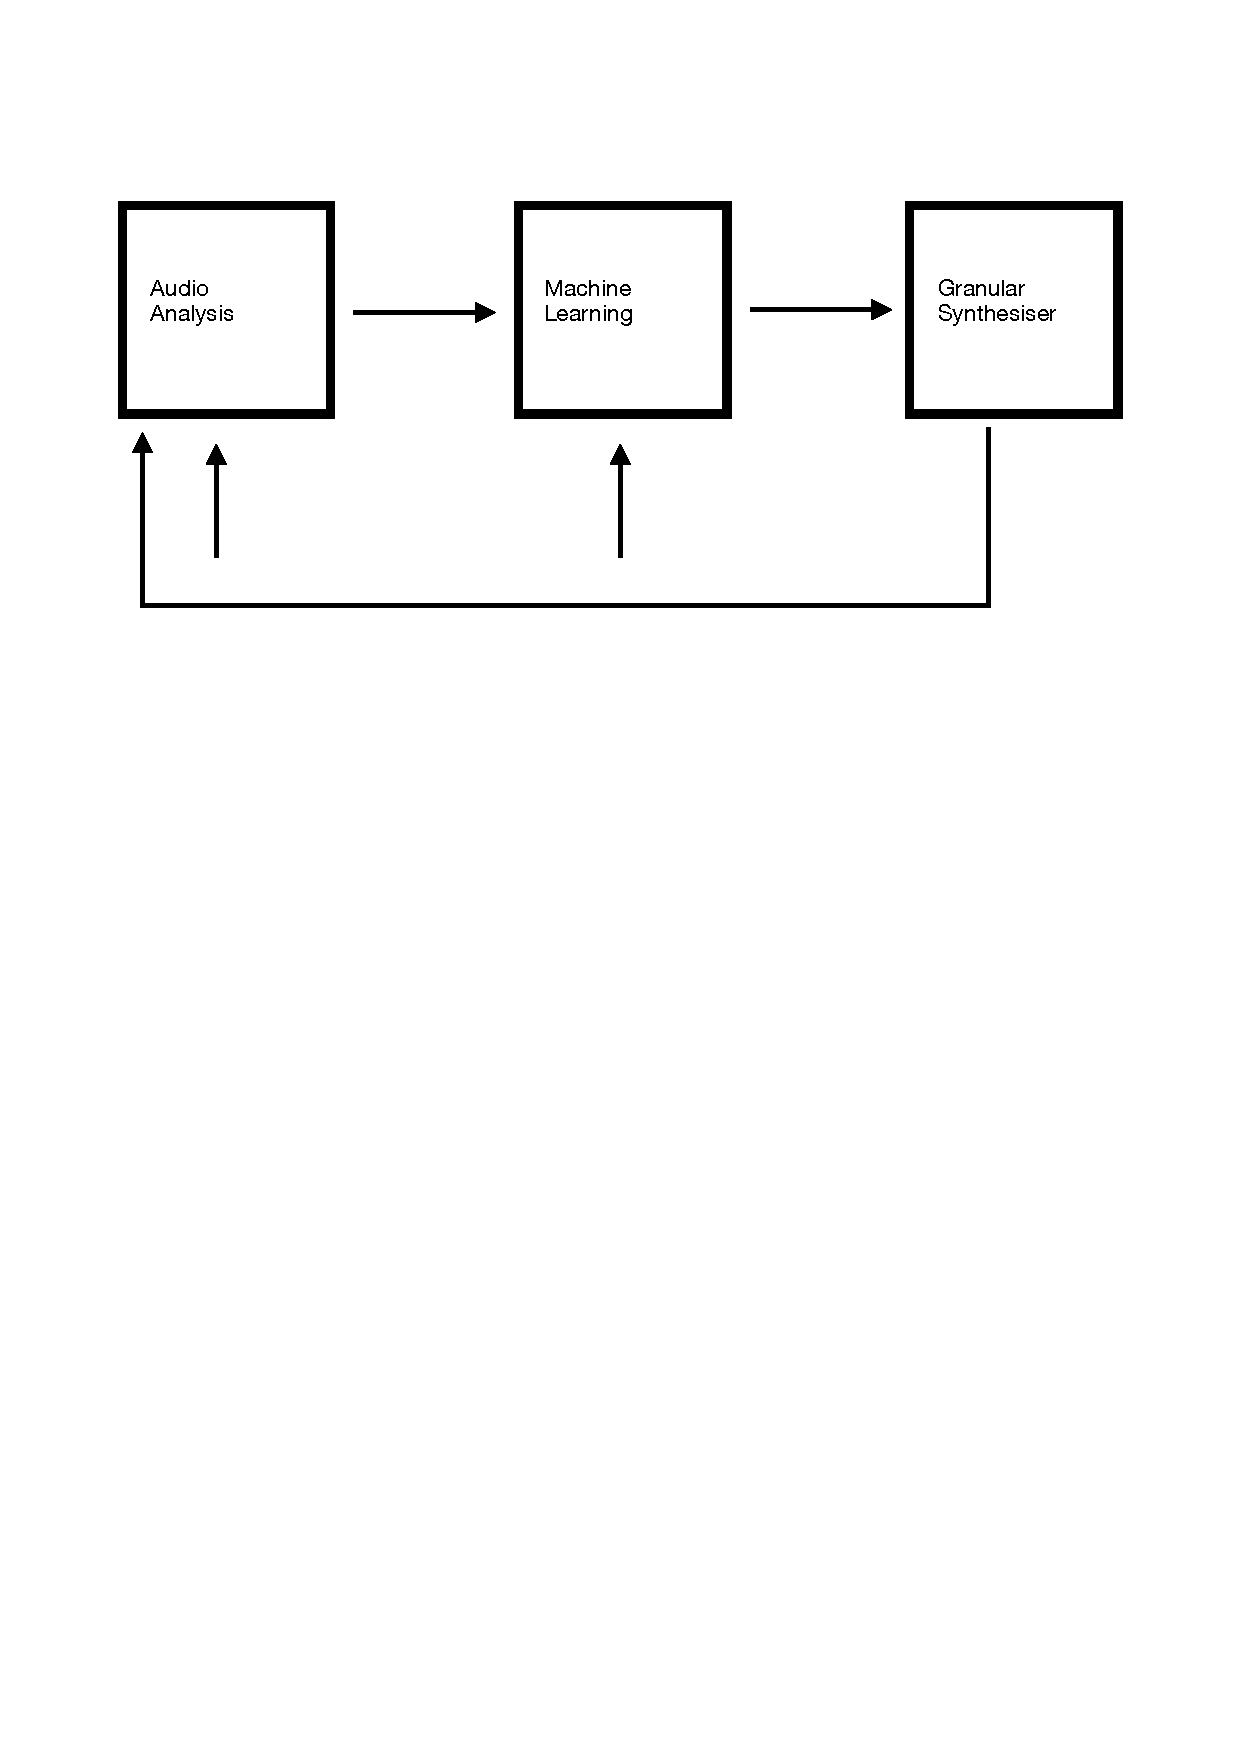
\includegraphics[width=0.5\textwidth]{images/flowchart}
\end{figure}

The box `Granular Synthesiser' in figure 1. represents a granular synthesizer.
It was implemented in C++, using the `JUCE' library.

`Machine Learning' stands for the predictions module, or more
precisely the Multilayer Perceptron model built in `Keras', and later
ported to C++ with the help of the `Frugally Deep' library.

Lastly, the `Audio Analysis' square represents the aspect of the
project responsible for extracting audio features from input
sounds. This was done with the `Essentia' library, that allowed me to
perform frame cutting, windowing, extracting the spectrum and finally
MFCCs on any specified buffer.

\section{Audio Analysis}

The only algorithm used for describing audio is the Mel-frequency
Cepstrum Coefficients. As mentioned in the Literature Review section,
it is proven to be one of the most reliable desriptors available, and
can not only describe the temporal qualities, but with the right
treatment, also be indicative of the changes that happen in the input
signal. More on that later.

In order to extract MFCCs from the signal, some preprocessing has to
be done. Namely, the signal has to be split into frames, on which the
FFT algorithm is performed. Each of the frames has to include a little
from the previous and the future one, in order to give a better
representaion of the signal. This is called a hop size.

Then, for each frame, MFCC are calculated based on the extracted
FFTs. The result for one frame is a vector of 13 floating point
values, each corresponding to a different range of frequencies.

At a sampling rate of 44.1kHz, and a buffer size of 512 samples, this
corresponds to exactly 45 vectors of 13 float values for one second of sound.

\section{Predictions}

\subsection{Dataset}

In order to get any predictions, a dataset, linking the MFCC values
with the synthesis parameters had to be created. Initially, I have set
out to create a data set of every possible combination of parameter
values, and their corresponding MFCCs. However, even though there are
only 5 adjustable parameters, with a static hop size of a tenth of
each parameter, it would take more than 1000 hours to complete this
task, given that each parameter combination would be sampled for
exactly one second.

In order to evade this limitation, a different approach was
taken. Every second, each parameter was set to a random value between
their unique minimum and maximum values. Consequently, the audio
features were extracted on each of these iterations, for exactly 10000
instances, which allowed for a creation of a dataset, of 10000
different parameter values, each corresponding to 10000 2D vectors, of
size 45 x 13 each.
%\cite{yee-king_automatic_2018}.

\subsection{Feedforward neural network}

The neural network implemented for the task of predicting the
synthesizer parameters is a Multilayer Perceptron. It's a relatively
simple, feedforward network, consiting of 3 layers.  The 45x13 MFCC
vectors served as the features, and a vector of 5 different parameter
values as the values to be predicted by the network. Firstly, the 2D
vectors, were flattened, like an image would be in a convolutional network.

Trained for 2000 epochs...
accuracy of 50\%...
parameters = this and that...
pretty shit, and not working very well, put not enough time for more experimentation...

\section{Synthesis}

\subsection{Granular Synthesis (basic explenation of the granular synth concept)}

Describing granular synthesis in one paragraph is impossible
without cutting some edges, and leaving out many intricacies of the
technique. However, a summary of sorts, describing the main concepts
behind the algorithm will be attempted here. 

Granular synthesis is an algorithm...
Grain clouds...
Xenakis...
Rodes...
Some other folks...
Capable of many thing, versatile...
graphs, graphs, graphs and pictures...

\subsection{The JUCE implementation (author's implementation)}

The granular synthesis algorithm was implemented using the `JUCE'
library. It is one of the most established libraries in the
professional audio community, being used by companies such as `Cycling
74', and `Korg' amog others(cite website?). On top of all things
audio, it provides a convenient way of creating a graphical user
interface, which was an important part of this project. Thanks to
`JUCE', the implementation was kept minimal, and elegant.

explenation of implementation...
grain class...
how grains are called...
how they are altered by the dials...
show code snippets...

\subsection{Synthesizer parameters}

There are 6 adjustable parameters...
position...
** where to spawn new grains
grain size...
** how the long are the grains spawned
position offset...
** how far away from the original position should the grains be spawned
number of grains...
** how many grain should be active at one point in time
pitch...
** how higher lower the pitch of each grain should be relative to the
original sample
global gain...
...





%What belongs in the "methods" section of a scientific paper?
%
%    Information to allow the reader to assess the believability of your results.
%    Information needed by another researcher to replicate your experiment.
%    Description of your materials, procedure, theory.
%    Calculations, technique, procedure, equipment, and calibration plots. 
%    Limitations, assumptions, and range of validity.
%    Desciption of your analystical methods, including reference to any specialized statistical software. 
%
%The methods section should answering the following questions and caveats: 
%
%    Could one accurately replicate the study (for example, all of the optional and adjustable parameters on any sensors or instruments that were used to acquire the data)?
%    Could another researcher accurately find and reoccupy the sampling stations or track lines?
%    Is there enough information provided about any instruments used so that a functionally equivalent instrument could be used to repeat the experiment?
%    If the data are in the public domain, could another researcher lay his or her hands on the identical data set?
%    Could one replicate any laboratory analyses that were used? 
%    Could one replicate any statistical analyses?
%    Could another researcher approximately replicate the key algorithms of any computer software?
%
%Citations in this section should be limited to data sources and references of where to find more complete descriptions of procedures.
%Do not include descriptions of results. % methods
\chapter{Results and Analysis}
\label{chapterlabel4}
\iffalse
    The results are actual statements of observations, including statistics, tables and graphs.
    Indicate information on range of variation.
    Mention negative results as well as positive. Do not interpret results - save that for the discussion. 
    Lay out the case as for a jury. Present sufficient details so that others can draw their own inferences and construct their own explanations. 
    Use S.I. units (m, s, kg, W, etc.) throughout the thesis. 
    Break up your results into logical segments by using subheadings
    Key results should be stated in clear sentences at the beginning of paragraphs.  It is far better to say "X had significant positive relationship with Y (linear regression p<0.01, r^2=0.79)" then to start with a less informative like "There is a significant relationship between X and Y".  Describe the nature of the findings; do not just tell the reader whether or not they are significant. 

Note: Results vs. Discussion Sections
Quarantine your observations from your interpretations. The writer must make it crystal clear to the reader which statements are observation and which are interpretation. In most circumstances, this is best accomplished by physically separating statements about new observations from statements about the meaning or significance of those observations. Alternatively, this goal can be accomplished by careful use of phrases such as "I infer ..." vast bodies of geological literature became obsolete with the advent of plate tectonics; the papers that survived are those in which observations were presented in stand-alone fashion, unmuddied by whatever ideas the author might have had about the processes that caused the observed phenomena.
 
How do you do this? 

    Physical separation into different sections or paragraphs.
    Don't overlay interpretation on top of data in figures. 
    Careful use of phrases such as "We infer that ".
    Don't worry if "results" seem short.

Why? 

    Easier for your reader to absorb, frequent shifts of mental mode not required. 
    Ensures that your work will endure in spite of shifting paradigms.
\fi% results and analysis
\chapter{Discussion}
\label{chapterlabel5}
\section{Summary of Findings}
\section{Evaluation}
\section{Future Work}

Start with a few sentences that summarize the most important results. The discussion section should be a brief essay in itself, answering the following questions and caveats: 

    What are the major patterns in the observations? (Refer to spatial and temporal variations.)
    What are the relationships, trends and generalizations among the results?
    What are the exceptions to these patterns or generalizations?
    What are the likely causes (mechanisms) underlying these patterns resulting predictions?
    Is there agreement or disagreement with previous work?
    Interpret results in terms of background laid out in the introduction - what is the relationship of the present results to the original question?
    What is the implication of the present results for other unanswered questions in earth sciences, ecology, environmental policy, etc....?
    Multiple hypotheses: There are usually several possible explanations for results. Be careful to consider all of these rather than simply pushing your favorite one. If you can eliminate all but one, that is great, but often that is not possible with the data in hand. In that case you should give even treatment to the remaining possibilities, and try to indicate ways in which future work may lead to their discrimination.
    Avoid bandwagons: A special case of the above. Avoid jumping a currently fashionable point of view unless your results really do strongly support them. 
    What are the things we now know or understand that we didn't know or understand before the present work?
    Include the evidence or line of reasoning supporting each interpretation.
    What is the significance of the present results: why should we care? 

This section should be rich in references to similar work and background needed to interpret results. However, interpretation/discussion section(s) are often too long and verbose. Is there material that does not contribute to one of the elements listed above? If so, this may be material that you will want to consider deleting or moving. Break up the section into logical segments by using subheads. % discussion
\chapter{Conclusion}

%    What is the strongest and most important statement that you can make from your observations? 
%    If you met the reader at a meeting six months from now, what do you want them to remember about your paper? 
%    Refer back to problem posed, and describe the conclusions that you reached from carrying out this investigation, summarize new observations, new interpretations, and new insights that have resulted from the present work.
%    Include the broader implications of your results. 
%    Do not repeat word for word the abstract, introduction or discussion.

\addcontentsline{toc}{chapter}{Appendices}

% The \appendix command resets the chapter counter, and changes the chapter numbering scheme to capital letters.
%\chapter{Appendices}
\appendix
\chapter{An Appendix About Stuff}
\label{appendixlabel1}
(stuff)

\chapter{Another Appendix About Things}
\label{appendixlabel2}
(things)

\chapter{Colophon}
\label{appendixlabel3}
\textit{This is a description of the tools you used to make your thesis. It helps people make future documents, reminds you, and looks good.}

\textit{(example)} This document was set in the Times Roman typeface using \LaTeX\ and Bib\TeX , composed with a text editor. 
 % description of document, e.g. type faces, TeX used, TeXmaker, packages and things used for figures. Like a computational details section.
% e.g. http://tex.stackexchange.com/questions/63468/what-is-best-way-to-mention-that-a-document-has-been-typeset-with-tex#63503

% Side note:
%http://tex.stackexchange.com/questions/1319/showcase-of-beautiful-typography-done-in-tex-friends 
% You could separate these out into different files if you have
%  particularly large appendices.

% This line manually adds the Bibliography to the table of contents.
% The fact that \include is the last thing before this ensures that it
% is on a clear page, and adding it like this means that it doesn't
% get a chapter or appendix number.
\addcontentsline{toc}{chapter}{Bibliography}

% Actually generates your bibliography.
\bibliography{example}

% All done. \o/
\end{document}